\begin{figure}[h]
  \centering
  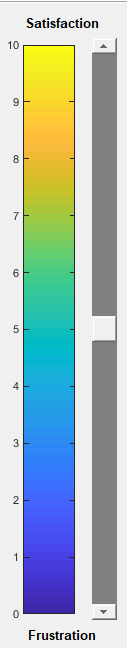
\includegraphics[width=\textwidth]{./Chapitre4/figures/satisfactionAxis.png}
  \caption{L'axe de satisfaction va de la frustration à la satisfaction, en passant par le neutre. C'est donc sur cet axe que l'annotation a été effectuée.}
  \label{fig:satisfactionAxis}
\end{figure}
